%\documentclass[prl,nofootinbib,twocolumn,floatfix,showpacs]{revtex4}
%\documentclass[manuscript]{revtex4}
\documentclass{article}
\usepackage{graphicx}
\usepackage{amsmath}
\usepackage{amssymb}

\begin{document}
\title{Anharmonicity and mode-coupling in a fluctuating protein}

\author{}
%\email{akabakcioglu@ku.edu.tr}
%\affiliation{Ko\c c University, Sar\i yer 34450 \. Istanbul, Turkey}

%\date{\today }

\begin{abstract}
We here develop a general framework for the residue
fluctuations that simultaneously incorporates both anharmonicity and
mode-coupling in a unified formalism. We show that both deviations
from the pure Gaussian model are important for modeling the
multidimensional energy landscape in the vicinity of the native state,
even at physiological conditions where fluctuations are relatively
small. (at what temperature is the MD?)

%%   I review the expansion of a multivariate probability distribution in terms
%%   of tensor Hermite polynomials and then discuss how the anharmonic terms of
%%   the form $x_1^\alpha x_2^\beta$ can be calculated in terms of the
%%   expectation values $\langle x_1^ix_2^j\rangle$. The result reduces the
%%   problem to calculation of Hermite polynomials $H_n(q)$ in one dimension, the
%%   coefficients of which one can write down in closed form. The method can be
%%   generalized to include three-point correlations $\langle x_1^ix_2^jx_3^k\rangle$.
\end{abstract}

%\pacs{}

\maketitle

\section{Introduction}
Residue fluctuations of a protein around its native state reveal
information that bridges the molecule's structural and functional
properties.  At the lowest order, these fluctuations can be treated as
a collection of independent harmonic modes, yielding ``Elastic Network
Models''~\cite{ENM}. However, it was recently shown that the slowest
oscillatory modes of a protein are strongly
anharmonic~\cite{Yogurtcu}, in contrast with the assumption underlying
ENMs. The coupling between different modes is another aspect of
protein dynamics that is believed to be relevant for the
information/energy transfer between different parts of the
molecule~\cite{mode_coupling_ref} and not captured by the harmonicity
assumption...

\section{Equilibrium fluctuations}

\subsection{Beyond Gaussian: the Hermite expansion}
Sampling the time evolution of a protein by using molecular dynamics
reveals a multivariate probability distribution function $f({\bf\Delta
  R})$ for the deviations of atoms (assume there are $N$ of them) from
equilibrium coordinates, i.e. $\Delta R_i = R_i - R_i^{eq}$,
$i=1,\dots,3N$. We here adopt a coarse-grained representation of this
p.d.f., where only $C_\alpha$ atoms are considered; i.e., $N$ is the
number of residues. Since the deviations from the free energy minimum
should be harmonic for sufficiently small amplitudes, Hermite
polynomials, which have a Gaussian kernel, constitute a natural basis
for representing $f({\bf\Delta R})$. First, following
Ref.~\cite{Yogurtcu}, we perform the transformation
\begin{eqnarray}
\label{eq:rotation}
{\bf \Delta r} &=& \langle {\bf\Delta R \Delta R}^T\rangle ^{-1/2} {\bf
  \Delta R}
\end{eqnarray}
which diagonalizes the covariance matrix $
Gamma\equiv\langle {\bf\Delta R \Delta R}^T\rangle$  and would give the normal
modes of the protein if fluctuations were harmonic. Otherwise, the
distribution function for $\{\Delta r\}$ in its most general form, can
be expressed as~\cite{Flory}
\begin{eqnarray}
\label{hermite_expansion}
f({\bf\Delta r}) &=& \frac{1}{\sqrt{(2\pi)^{3N}}} e^{
    -{\sum_{i=1}^{3N} \Delta r_i^2}/2} \bigg[ 1 +  \sum_{\nu=3}^\infty
 {\bf C_\nu}\cdot {\bf H}_\nu({\bf \Delta r}) \bigg]
\end{eqnarray}
where ${\bf C}_\nu$ (constant) and ${\bf H}_\nu$ (derived below) are
tensors of rank $\nu$, and the dot product refers to
$\sum_{ij..k}\,C_\nu^{ij..k}\,H_\nu^{ij..k}$.  The fluctuations in
this ``normal'' basis are meanless, i.e., $\langle {\Delta r_i}\rangle
= 0$, and decoupled at the lowest (second) order, i.e.,
\begin{equation}
\langle {
\label{eqn:pair_corr}
  \Delta r_i^T \Delta r_j}\rangle = \delta_{ij}\ .
\end{equation}
A purely harmonic model is given by ${\bf C}_\nu = 0,\ \forall \nu$.

As a reminder to the reader, tensor Hermite polynomials can be
obtained by successive differentiation using Rodrigues' formula:
\begin{eqnarray}
\label{Rodrigues}
H_{\nu}^{ij..k}({\bf \Delta r}) &=& \frac{(-1)^\nu}{g({\bf
    \Delta r})}\,{\bf\nabla}^{ij..k}\,g({\bf \Delta r})\ .
\end{eqnarray}
Above, $g({\bf x}) = (2\pi)^{3N/2}\exp(-{\bf x}^2/2)$ is the
multi-dimen{\-}sional Gaussian distribution and ${\bf \nabla}^{ij..k} =
\nabla^i\nabla^j\,..\,\nabla^k$ is the gradient tensor with
$\nabla^i \equiv \partial/\partial x_i$. Explicitly,
\begin{eqnarray}
{\bf H}^{ij}_2({\bf \Delta r}) &=& \Delta r_i\Delta r_j - \delta_{ij} \nonumber \\
{\bf H}^{ijk}_3({\bf \Delta r}) &=& \Delta r_i\Delta r_j\Delta r_k - \delta_{ij}\Delta r_k- \delta_{jk}\Delta r_i- \delta_{ki}\Delta r_j \nonumber \\
& \cdots &
\end{eqnarray}
where $i$, $j$, $k$ run over the components of the vector ${\bf\Delta
  r}$. Higher order Hermite polynomials can be obtained by summing all
possible $0,1,.., \lfloor\frac{\nu}{2}\rfloor$ pairwise
contractions ($\delta_{ij}$s)  of $\Delta r_i\Delta r_j\,..\,\Delta r_k$, a minus sign
accompanying the terms obtained by an odd number of
contractions. Diagonal elements of ${\bf H}_\nu$ (corresponding to a
scalar $\Delta r$) are the usual Hermite polynomials
\begin{eqnarray}
H_\nu(\Delta r) &=& \sum_{m=0}^{\nu/2} (-1)^m\, {\nu \choose 2m} \,m!!\,\Delta r^{\nu-2m}
\label{hermite_anal}
\end{eqnarray}
where $m!!\equiv \frac{(2m)!}{2^m m!} = (2m-1)(2m-3)\cdots 3\cdot
1$, and the combinatorial expression counts the number of $m$ pairwise
contractions of $\nu$ variables.

The orthogonality condition for the Hermite tensor polynomials,
\begin{eqnarray}
\label{orthogonality}
\int_{-\infty}^{\infty}{\bf dx}\, \big[{\bf A}_\nu\cdot {\bf H}_\nu({\bf x})\big] {\bf
  H}_\mu({\bf x})e^{-{\bf x}^2/2} &=& \begin{cases}{\bf A}_\nu\nu !\ , & \nu=\mu
  \\ 0\ , & \nu\neq\mu \end{cases}
\end{eqnarray}
is true for any constant tensor ${\bf A}_\nu$ of rank $\nu$.  In
particular, the tensor coefficients that appear in $f({\bf \Delta r})$
follow from the orthogonality relation as
\begin{eqnarray}
\label{coefs}
{\bf C}_\nu &=& \frac{1}{\nu!}\int_{-\infty}^{\infty} {\bf H}_\nu({\bf x})
f({\bf\Delta r})\, {\bf d\Delta r} =  \langle {\bf H}_\nu({\bf\Delta r})\rangle/\nu!
\end{eqnarray}
Therefore, the problem reduces to obtaining the expectation values of
the polynomial tensor elements for the system. At the lowest
nonvanishing order they read
\begin{eqnarray}
\label{H3}
%% {\bf H}_2^{11}({\bf x}) &=& x_1^2 - 1 \nonumber \\
%% {\bf H}_2^{12}({\bf x}) &=& x_1x_2 \nonumber \\
{\bf H}_3^{111}({\bf x}) &=& x_1^3 -3x_1 \nonumber \\
{\bf H}_3^{112}({\bf x}) &=& x_1^2x_2 -x_2 = {\bf H}_3^{121}({\bf x}) = {\bf
  H}_3^{211}({\bf x}) \nonumber \\
{\bf H}_3^{123}({\bf x}) &=& x_1x_2x_3
\end{eqnarray}
and some of the next order tensor elements are:
\begin{eqnarray}
\label{H4}
{\bf H}_4^{1111}({\bf x}) &=& x_1^4 -6x_1^2 + 3 \nonumber \\
{\bf H}_4^{1112}({\bf x}) &=& x_1^3x_2 - 3x_1x_2 \nonumber \\
&=& {\bf H}_3^{1121}({\bf x}) = {\bf H}_3^{1211}({\bf x}) = {\bf  H}_3^{2111}({\bf x}) \nonumber \\
{\bf H}_4^{1122}({\bf x}) &=& x_1^2x_2^2 - x_1^2 - x_2^2 + 1 \nonumber \\
&=& {\bf H}_4^{1212}({\bf x}) = {\bf  H}_4^{1221}({\bf x}) \nonumber \\
{\bf H}_4^{1123}({\bf x}) &=& x_1^2x_2x_3 - x_2x_3  = {\bf H}_4^{1231}({\bf x}) = {\bf H}_4^{1213}({\bf x}) = \cdots
\end{eqnarray}
A graphical representation of $H_4$ in one and two dimensions is given in Fig.\ref{Fig1}. 
\begin{figure}
\vspace*{2cm}
  \begin{center}
    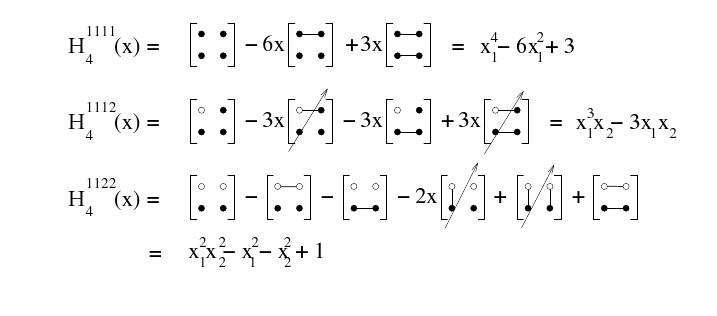
\includegraphics[width=10cm]{./Fig1.jpg}
  \end{center}
\caption{Graphical representation of $H_4(x)$ tensor elements in two
dimensions. Terms that vanish by virtue of Eq.~(\ref{eqn:pair_corr})
are crossed with an arrow.}
\label{Fig1}
\end{figure}


The inclusion of mode-coupling necessitates consideration of mixed
indices (nondiagonal tensor elements). Here, we focus on the coupling
between mode pairs and ignore threesome and higher order mixing, i.e.,
we consider only the bi-polynomials ${\bf H}^{i_1i_2\dots
  i_\nu}_\nu(\Delta r_k,\Delta r_l)$ with $i_m \in \{k,l\}$,
$k,l=1,2,\dots,3N$. At first sight, estimating the contribution of
mode-coupling even at this lowest level appears to be a formidable
task, because for the optimal cut-off rank $\nu=16$ (see below), the
number of distinct expectation values to be extracted from the data
grows combinatorially. We show below that, the factorization property
of the off-diagonal tensor elements and the orthogonality of the modes
at the second order bring a significant reduction in complexity, which
we exploit to investigate the impact of anharmonicity and
mode-coupling separately on the protein dynamics.

\subsection{Mode-coupling corrections}
In order to reach the desired formulation, we first note that the value
of a tensor element ${\bf H}^{i_1i_2\dots i_\nu}_\nu({\bf \Delta r})$
does not depend on the order of the indices due to the commutativity
of the gradient operator, $\nabla_k\nabla_l -
\nabla_l\nabla_k=0$. Therefore,
\begin{eqnarray}
{\bf H}^{i_1i_2\dots i_\nu}_\nu({\bf \Delta r}) &=& {\bf H}^p_\nu(\Delta r_k,\Delta r_l) \nonumber
\end{eqnarray}
where $p$ is the number of indices equal to $k$ (and the remaining
$\nu-p$ indices are equal to $l$). The fact that the covariance matrix
in $\{{\bf \Delta r}\}$ basis is diagonal further implies that
\begin{eqnarray}
\label{factorization}
{\bf H}^p_\nu({\bf \Delta r}) &=& H_p(\Delta r_1)\times H_{\nu-p}(\Delta r_2)
\end{eqnarray}
as is also evident from the Rodrigues's formula in Eq.~(\ref{Rodrigues}).

Combining Eqs.(\ref{coefs})\&(\ref{factorization}), the Hermite
expansion in Eq.~(\ref{hermite_expansion}) can be cast into the
following form:
\begin{eqnarray}
\label{hermite_expansion2}
f({\bf\Delta r}) &=& \frac{1}{\sqrt{(2\pi)^N}} e^{ -\sum_i \Delta
  r_i^2/2} \bigg[ 1 + \sum_i\sum_{\nu=3}^\infty
  \frac{1}{\nu!}\, \Big\langle
  H_\nu(\Delta r_i)\Big\rangle\,H_\nu(\Delta r_i) \nonumber \\
&+&  \sum_{i\ne j}\sum_{\nu=3}^\infty
  \frac{1}{\nu!}\,\sum_{p=1}^{\nu-1} {\nu\choose p} \Big\langle
  H_p(\Delta r_i)H_{\nu-p}(\Delta r_j)\Big\rangle\,H_p(\Delta r_i)H_{\nu-p}(\Delta r_j) \nonumber \\
&& + \sum_{i\ne j\ne k} \cdots \bigg]
\end{eqnarray}
The first term in $[\cdots]$ corresponds to a purely harmonic given by
the Gaussian probability distribution
\begin{eqnarray}
\label{eqn:f0}
f_0({\bf\Delta r}) &=& \frac{1}{\sqrt{(2\pi)^N}} e^{ -\sum_i \Delta
  r_i^2/2}\ .
\end{eqnarray}
This is the starting point for most of the past studies on protein
fluctuations\cite{}. The next in Eq.~(\ref{hermite_expansion2}) term is
appreciable when the modes are anharmonic, but gives no information
about mode-coupling. In fact, the most general mode-amplitude
distribution of an anharmonic model composed of decoupled modes is
\begin{eqnarray}
\label{decoupled}
f_1({\bf\Delta r}) &=& \frac{1}{\sqrt{(2\pi)^N}}\ e^{ -\sum_i \Delta
  r_i^2/2}\times \prod_i \bigg[ 1 + \sum_{\nu=3}^\infty
  \frac{1}{\nu!}\, \Big\langle
  H_\nu(\Delta r_i)\Big\rangle\,H_\nu(\Delta r_i)\bigg] \nonumber \\
&&
\end{eqnarray}
The approximation to the true distribution given in
Eq.~(\ref{decoupled}) is named $f_1$ in order to remind the reader
that it qualitatively improves on the Gaussian approximation $f_0$
of Eq.~(\ref{eqn:f0}). The difference between the full pdf given in
Eq.~(\ref{hermite_expansion2}) and the approximation $f_1$ is the
mode-coupling corrections such as
\begin{eqnarray}
\langle H_p(\Delta r_i)H_{\nu-p}(\Delta r_j)\rangle - \langle
H_p(\Delta r_i)\rangle\langle H_{\nu-p}(\Delta r_j)\rangle &\neq& 0 \nonumber
\end{eqnarray}
and higher order cumulants. Note that, these corrections are transparent to the
marginal distributions
\begin{eqnarray}
\label{marginal}
f(\Delta r_i) &\equiv& \int_0^\infty \prod_{j\ne i}d\Delta r_j\ f({\bf\Delta r})\ 
\end{eqnarray}
as a merit of the orthogonality relation in
Eq.~(\ref{orthogonality}). Therefore, even if the marginal
distributions are reproduced to good accuracy, the multi-dimensional
free-energy landscape of the protein may still be very different from
that implied by a model based on Eq.~(\ref{decoupled}). We demonstrate
below that this is the case for the protein Crambin 2CI2. To this end,
we improve the approximation in Eq.~(\ref{decoupled}) one step
further and set $f({\bf\Delta r})$ to
\begin{eqnarray}
\label{hermite_expansion2}
f_2({\bf\Delta r}) &=& \frac{1}{\sqrt{(2\pi)^N}} e^{ -\sum_i \Delta
  r_i^2/2} \bigg[ 1 + \sum_i\sum_{\nu=3}^\infty
  \frac{1}{\nu!}\, \Big\langle
  H_\nu(\Delta r_i)\Big\rangle\,H_\nu(\Delta r_i) \nonumber \\
&+&  \sum_{i\ne j}\sum_{\nu=3}^\infty
  \frac{1}{\nu!}\,\sum_{p=1}^{\nu-1} {\nu\choose p} \Big\langle
  H_p(\Delta r_i)H_{\nu-p}(\Delta r_j)\Big\rangle\,H_p(\Delta r_i)H_{\nu-p}(\Delta r_j) \bigg] \nonumber \\
&&
\end{eqnarray}
which takes into account the mode-coupling corrections at the lowest
order they appear and ignores higher-order terms cubic in $H_\nu$.
In the next section, we present our results for Crambin.



\section{Experiment}

\subsection{The Simulation}

Crambin (Protein Data bank code 1EJG.pdb) was selected as an example
since it is a relatively small protein and its dynamics is
widely studied \cite{Teeter1990,Levitt1985,Lange2006}.  
{\bf Need to get the references from ``MD EXPERIMENTS.DOC''}

{\it THIS PART COULD GO TO THE SUPPLEMENTS MAYBE?\\
All Molecular dynamics simulations were performed for an N,P,T
ensemble in explicit solvent (water) at 310 K using NAMD 2.5 package
with CHARMM27 force field. The protein was solvated in a waterbox of
15 A cushion and periodic boundary conditions were applied. Ions were
added in order to represent a more typical biological
environment. Langevin dynamics was used to control the system's
temperature and pressure. All atoms were coupled to the heat bath of
temperature of 310 K. A time step of 1fs was used. Nonbonded and
electrostatic forces were evaluated each time step. In order to keep
all degrees of freedom no rigid bonds were used.

We used two minimization-equilibration cycles: The first one was
applied to relax the water in the first place and the second one was
applied to find a local minimum of the whole system’s energy
\cite{NAMD2009}. The energy of the initial system was first minimized
for 20000 steps. The system was then equilibrated by first keeping the
Protein fixed for the first 0.1 ns. It took 0.02ns for the volume to
converge. During the remaining 0.08ns volume fluctuated around 159000
$\mbox{Angstrom}^3$. Then, the protein was released stepwise by
applying harmonic constraining forces to every backbone atom of 1, 0.5
and 0.25 kcal/(mol*$\mbox{Angstrom}^2$) in magnitude each for 0.05
ns. Finally the simulation was performed for an additional 0.05ns
without applying any force. Having finished the first cycle, the
second minimization-equilibration cycle was performed, this time the
protein was free to move. Again 20000 steps of minimization were
applied and system was equilibrated for 6ns.
%%% (Hocam bu yaklaşık olarak. Kesin aldığım zamanı hatırlayamıyorum). 
At every 100th time step, the instantaneous atomic coordinates
$\hat{R}$ of all atoms, the velocities, the pressures and the energies
were recorded. A 0.9 ns long part of the trajectory consisting of 9000
frames was used. In order to eliminate all the rotational and
translational motions, all structures were aligned with respect to the
initial structure using the transformation matrix which shows the best
mass weighted fit with the initial structure. All transformation
matrices were constructed via TCL commands in VMD.}

The 46 residue Crambin consists of 657 atoms. Taking only the alpha
carbons into account a set of 138 modes were obtained. Then the
overall rotational and translational motions were eliminated since
they are irrelevant for the internal motion \cite{Moritsugu2003}. All
structures were translated so that their center of mass is positioned
at the origin and rotated to obtain the best mass weighted RMSD fit
with the initial structure.

The fluctuation ${\bf \Delta R}$ of atoms are defined by ${\bf \Delta
R} = {\bf {R}-\bar{R}}$, where ${\bf \bar{R}}$ are the mean atomic
coordinates and hence is a time independent quantity, which defines an
average configuration obtained by the protein during the part of the
trajectory that we use for calculations. The potential energy of this
mean configuration is $V_0$. In the remaining sections of the paper we
characterize the deviations of the potential energy of the residues
from that of the reference conformation.

%% The covariance matrix $C$ is defined in terms of $\Delta R$ as

%% \begin{equation} \label{eqn:C}
%% C = \left< \Delta R \Delta R^T \right>
%% \end{equation}

%% Here, the angular brackets denote the average, taken over the
%% trajectory.

The instantaneous fluctuations are transformed into modal space using
Eq.~(\ref{eq:rotation}) where the average denoted by the angular
brackets is taken over the trajectory. \cite{Amadei1993,Yogurtcu2009}.
%% \begin{equation} \label{eqn:r}
%% \Delta r = C^{-1/2} \Delta R
%% \end{equation}
%% where $\Delta r$ are the dimensionless transformed fluctuations in
%% modal space.
We let $e$ represent the eigenvector matrix that diagonalizes
$\Gamma^{-1/2} = \left<{\bf \Delta R \Delta R^T} \right>^{-1/2}$, and
$\lambda$ represent the eigenvalues. Then, $\Gamma^{-1/2}= \mbox{diag }
\lambda^{-1/2}\, e^T$ and the fluctuations ${\bf \Delta r}$ are the
fluctuations in mode space spanned by the eigenvectors, $e$
\cite{Yogurtcu2009}. The components of the real trajectory that
correspond to a given mode is obtained simply by keeping the
eigenvalue of interest, equating all the others to zero, followed by a
back transformation of Eq.~(\ref{eq:rotation}).

\subsection{Dataset}

%% This should probably be merged with the above section.

The full dataset consists of 8967 snapshots of 132 modes.  To prevent
overfitting, every 9-th snapshot (a total of 996) was reserved as the
test set and the rest (7971 snapshots) were used as the training set.
%% 8967b.dat, 8967b.tst.dat, 8967b.trn.dat
Because of normalization, each mode has zero mean and unit variance.
Figure~\ref{fig:timeplots} gives the time plots of a few of the sample
modes.  

%% timeplots.gp, 8967b.dat

\begin{figure}[h]
  \includegraphics[width=.5\textwidth]{src/mode01.pdf}
  \includegraphics[width=.5\textwidth]{src/mode05.pdf} \\
  \includegraphics[width=.5\textwidth]{src/mode10.pdf}
  \includegraphics[width=.5\textwidth]{src/mode50.pdf}
\caption{Time plots of sample modes.}
\label{fig:timeplots}
\end{figure}

\subsection{Baselines}		% F0, F1

In this section we introduce two baseline density models that do not
take into account mode coupling.  The first baseline model, $f_0$, is
the standard multivariate normal distribution with zero mean and unit
variance in Eq.~(\ref{eqn:f0}).  The second baseline model, $f_1$, uses
first-order hermite corrections based on statistics of the training
data given by Eq.~(\ref{decoupled}).

To compare the quality of the models, we use the average log
likelihood of the snapshots in the test data given parameters
optimized for the training data\footnote{except for $f_0$, which has
no parameters to optimize}.  Eq.~(\ref{eqn:logl}) defines the
average log likelihood of the data.  ${\bf\Delta r}^{(i)}$ denotes the
$i$'th snapshot and $N$ is the number of snapshots.

\begin{equation}
\label{eqn:logl}
\left< \log f({\bf\Delta r}) \right> = \frac{1}{N} \sum_{i=1}^N \log f({\bf\Delta r}^{(i)})
\end{equation}

The average log likelihood based on $f_0$ is -187.449 per snapshot,
corresponding to 111.5 kcal/mol contribution to the free energy at
room temperature ( $= \langle\log f\rangle k_B\times 1.6\cdot
10^{-19}\times 6.02\cdot 10^{23} / 4200$ - Alkan). The measurement of $f_1$ is a
bit more problematic because the approximation gives negative
probabilities on some test instances.  This problem can be partially
solved by applying the $f_1$ approximation only to the first few modes
and assuming the rest are coming from the standard normal
distribution.  Figure~\ref{fig:f1} describes the outcome based on the
number of modes where the $f_1$ approximation is applied.  The first
plot gives the average log likelihood based on only the positive
probability instances.  The second plot gives the proportion of
negative probability instances.  If we ignore the negative
probabilities the best log likelihood for $f_1$ is -186.43.

%% src/8967b.tst.f0.out
%% f1.sh f1analyze.pl f1analyze.out f1analyze.gp

\begin{figure}[h]
  \includegraphics[width=.5\textwidth]{src/f1logp.pdf}
  \includegraphics[width=.5\textwidth]{src/f1negp.pdf}
\caption{Log likelihood and proportion of negative probabilities given
  the number of modes where $f_1$ approximation is applied.}
\label{fig:f1}
\end{figure}

The slight improvement of $f_1$ over $f_0$ is due to the better fit
$f_1$ provides for individual modes.  Figure~\ref{fig:f1histogram}
compares the $f_0$ and $f_1$ distributions with the test data
histogram for mode 1.  Although $f_1$ fits the marginal mode
distributions better, modes are still assumed independent of each
other.

%% f1histogram.pl f1histogram.out f1histogram.gp f1histogram.pdf

\begin{figure}[h]\centering
  \includegraphics[width=.7\textwidth]{src/f1histogram.pdf}
\caption{A comparison of $f_0$ and $f_1$ with the normalized histogram for
  mode 1}
\label{fig:f1histogram}
\end{figure}

\subsection{Mode Coupling Corrections} % F2 ve mode coupling analysis

%% TODO: try 1-132 modes approximated by f2 -- running
%% TODO: get surface plots of f0, f1, f2 for modes 1-2
%% TODO: research mode coupling

The $f_2$ approximation (Equation~\ref{hermite_expansion2}) can model
pairwise interactions between modes.  Figure~\ref{fig:f2} shows the
log likelihood achieved and the proportion of negative probabilities
based on the number of modes $f_2$ approximation is applied.  The
remaining modes are assumed to be generated independently from the
standard normal distribution.  If we ignore the negative probabilities
the best log likelihood for $f_2$ is -180.05, {\it a correction of
$\approx 3.8$ kcal/mol to the free energy solely due to
mode-coupling.}(Bu free energy farki daha anlamli herhalde. -Alkan)

%% f2.sh f1analyze.pl f2analyze.out f2analyze.gp

\begin{figure}[h]
  \includegraphics[width=.5\textwidth]{src/f2logp.pdf}
  \includegraphics[width=.5\textwidth]{src/f2negp.pdf}
\caption{Log likelihood and proportion of negative probabilities given
  the number of modes where f2 approximation is applied.}
\label{fig:f2}
\end{figure}

$f_2$ achieves a significantly better fit to the data compared to
$f_1$.  The two models give identical marginal distributions to
individual modes.  The difference comes from $f_2$'s better modeling
of pairwise interactions.  Figure~\ref{fig:contour} compares $f_1$ and
$f_2$ distributions with the scatter plot of the first two modes.

\begin{figure}[h]
  \includegraphics[width=.5\textwidth]{src/f1contour.pdf}
  \includegraphics[width=.5\textwidth]{src/f2contour.pdf}
\caption{A comparison of $f_1$ and $f_2$ against a scatter plot of the
  first two modes.}
\label{fig:contour}
\end{figure}

\subsection{Kernel Density Estimation}

%% TODO: Compute kde results, generate surface plot for 1-2

To quantify the effects of phenomena beyond pairwise interactions, we
used non-parametric kernel density estimation (KDE) procedure to model
the probability density of the training set.  We fit second order
Gaussian kernels with fixed bandwidths optimized using likelihood
cross validation\footnote{We used the ``npudensbw'' and ``npudens''
  procedures with default arguments from the ``np'' package for the
  ``R'' statistical computing environment by Tristen Hayfield and
  Jeffrey S. Racine.}.

Figure~\ref{fig:kde} shows the log likelihood achieved based on the
number of modes KDE approximation is applied.  The remaining modes are
assumed to be generated independently from the standard normal
distribution.  There are no negative probability estimates in KDE.

\begin{figure}[h]\centering
  \includegraphics[width=.7\textwidth]{src/kdelogp.pdf}
\caption{Log likelihood given the number of modes where KDE
  approximation is applied.  Each curve represents a different
  training set size.  The best result is -176.569 using 30 modes on
  the full training set of 7971 instances.}
\label{fig:kde}
\end{figure}

Figure~\ref{fig:contour2} compares $f_2$ and KDE distributions with
the scatter plot of the first two modes.  KDE achieves a
significantly better fit to the data compared to $f_2$.  The peaks are
higher and the contours are more detailed for the KDE figure.  More
importantly KDE is not restricted to pairwise interactions only, it
can model higher order interactions as well.

\begin{figure}[h]
  \includegraphics[width=.5\textwidth]{src/f2contour.pdf}
  \includegraphics[width=.5\textwidth]{src/kdecontour.pdf}
\caption{A comparison of $f_2$ and KDE against a scatter plot of the
  first two modes.}
\label{fig:contour2}
\end{figure}

\begin{thebibliography}{99}

\bibitem{ENM}{ Reference GNM, ENM, etc.}
\bibitem{Yogurtcu}{ Yogurtcu {\it et al.} (2009).}
%% \bibitem{FPU}{Scholarpedia 3 (8) 5538 (2008) - Dauxois T and Ruffo S ``FPU nonlinear lattice
%% oscillations''}
\bibitem{mode_coupling_ref}{ Reference on mode coupling, enegry transfer between modes, etc.}
\bibitem{Flory}{Flory, 1976.}

\end{thebibliography}

\end{document}
